\section{The Logistic Map as Model for Population Growth}

One dimensional recursive equations $x_{n+1} = f(x_n)$ are used for modeling various dynamical systems. 
Its simplicity makes it easy to study, and many of its properties are also inherited by their more complicated counterparts.

Consider, for example, bacteria population in discrete time intervals. 
If the population is low and resource abundant, the rate of growth is in porportion to the population, which give rise to the following equation

$$
p_{t+1} = p_{t} b,
$$
where $p_{t}$ is the population of the bacteria at the dicrete time $t$ and $b$ as a constant is the static birth rate for bacteria whose value will depend on the model.

The limited resource will slow down the rate of growth as the population increases, and the the relation will become 

$$
	p_{t+1} =  p_{t} \be
$$

The usual assumption is that $\be$ is close to $b$ when the population is low, and there is a threshold which the population will never surpass. At the threshold $\be$ will be zero.

The simplest equation for modelling $\be$ is the linear equation

$$
\be = b - ap,
$$

where $a$ is another constant.
Combining the two, the recursive formula becomes 

$$
p_{t+1}  = b p_t - ap_t^2
$$

Substituting $p_{t} := \frac{b}{a} x_{t}, \lambda := \frac{b}{4}$, we obtain

$$
x_{t+1} = 4 \lambda x_t(1-x_t) 
$$

Indeed, thence come the standard forms of the logistic map

\begin{equation}\label{eq_logistic}
	L_{\lambda}(x) = 4 \lambda x(1-x)
\end{equation}

% graph produced by `logistic_map_diff_lambda`
\begin{figure}[t]
	\centering
	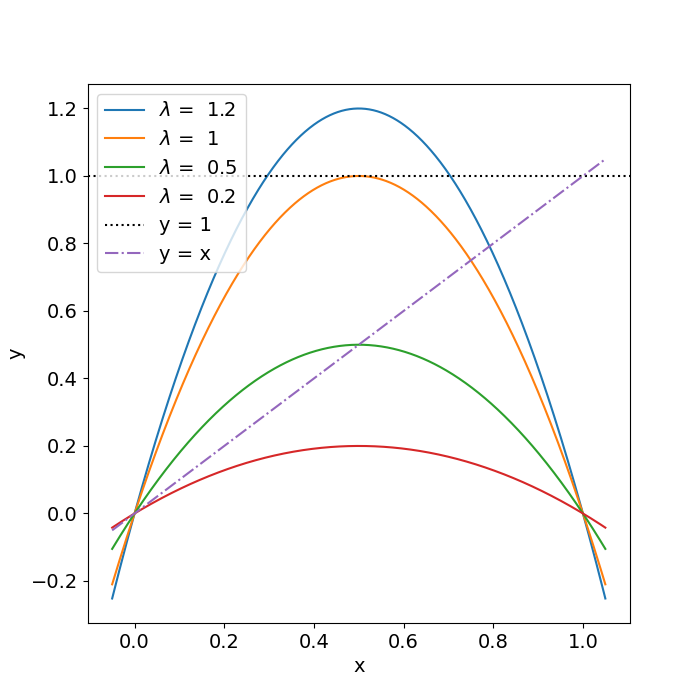
\includegraphics[width=0.7\textwidth]{./figures/logistic_map_diff_lambda.png}
	\caption{Graphs of logistic map $L_{\lambda}(x) = 4 \lambda x(1-x)$ for different $\lambda$ compared with the line $y=x$ and $y = 1$.} 
	\label{fig:logistic_map_diff_lambda}
\end{figure}


For our purpose the restriction $\lambda >0$ is applied.
Scrutinising the class of discrete logistic functions plotted in figure \ref{fig:logistic_map_diff_lambda}, some of their properties are obvious

\begin{enumerate}
	\item $\L(x)$ is a smooth function.
	\item $\L(x)$ concaves downwards, that is, $\L(x)'' < 0$.
	\item $\L(x)$ attains a unique maximum at $x = \frac{1}{2}$, and $L_{\lambda}(\frac{1}{2}) = \lambda$.
	\item When $0 \leq \lambda$ and $x$ is restricted to the domain $[0, 1]$, $\L(x)$ is a two-to-one non-surjective (except for $\lambda = 1$) function $\L(x): [0,1] \rightarrow [0,\lambda]$. 
\end{enumerate}

Some sources defined the logistic map as $L'_{\lambda'}(x) = \lambda' x(1-x)$ without the constant 4. 
In this report, however, we will use equation \ref{eq_logistic}, which has the advantage that the maximum value attained by $\L(x)$ is $\lambda$. This notation will also be consistent to the definitions of other class of functions discussed later in the report.

We can check if this model would work as expected by comparing it to its continuous counterpart 

\begin{equation}\label{eq_logistic_continuous}
	\frac{dp}{dx} = c p(x) (1-p(x)),
\end{equation}

whose unique solution with the initial condition $p(0) = \frac{1}{2}$ is 

$$
p(x) = \frac{e^{cx}}{1+e^{cx}}
$$

\begin{figure}[b!]
	\centering
	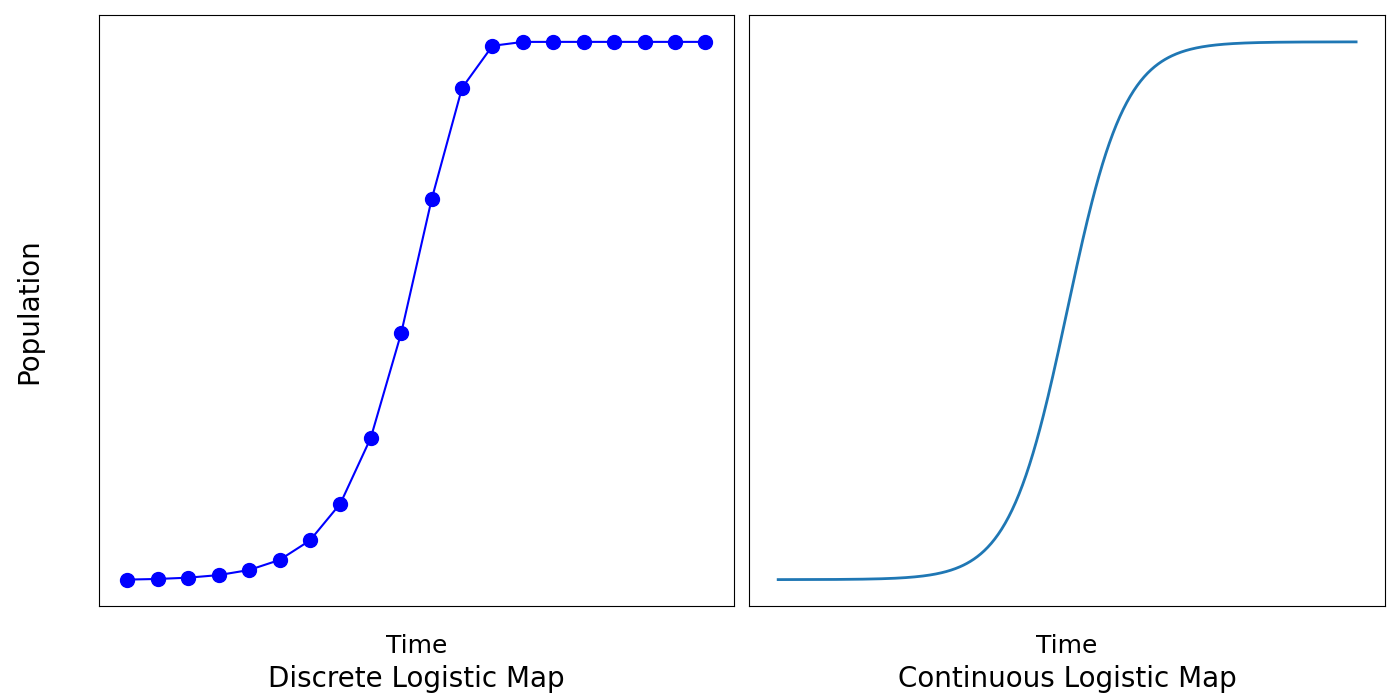
\includegraphics[width=0.8\textwidth]{./figures/con_vs_discrete_logistic_map.png}
	\caption{Discrete (left) v.s. continuous (right) logisitc map. Discrete case is modeld by $\lambda = 0.5$ and $x_0 = 0.0003$. The continuous case has $c=1$.}
	\label{fig:con_vs_discrete}
\end{figure}

The graph of these two maps are shown in figure \ref{fig:con_vs_discrete}.
The population of the discrete case was obtained by setting an arbitrary initial value, here $x_0 = 0.0003$, and the population of the next time interval was obtained by simple iteration of the logistic map, that is $x_{i+1} = L_{\lambda}(x_i)$.
For the continuous case the population at each time was obtained by solving the differential equation with initial condition.
Indeed, at least for the selected value of $\lambda$ and $c$, the population modeld by the two maps are similar.

Having settled that the discrete logistic map is indeed, at least for some values of $\lambda$, a good simplification for the already-simplified equation \ref{eq_logistic_continuous} as a model for population growth, you may wondered why bother studying such a simple equation. 
The reason is, as simple as it seems, the iteration of equation \ref{eq_logistic} gives rise to some extremely complicated dynamical systems with many surprising properities. 
These interesting dynamics are also observed in the continuous case and is the study of the next session.

% graph produced by logistic_vs_continuous_modelling_population


\section{Logistic Bifurcations}

The first step of studying logistic bifurcations is to plot it with different initial values and $\lambda$. 
For now only $0 \leq \lambda \leq 1$ and $0 \leq x_0 \leq 1$ are considered, so that $\L(x)$ is a map from $[0,1]$ to $[0,1]$. 

% graph produced by `modelling_pop_with_diff_logistic_maps` in `graph_qc` repo
\begin{figure}[htbp]
	\centering
	\label{fig:various_iter_logistic}
	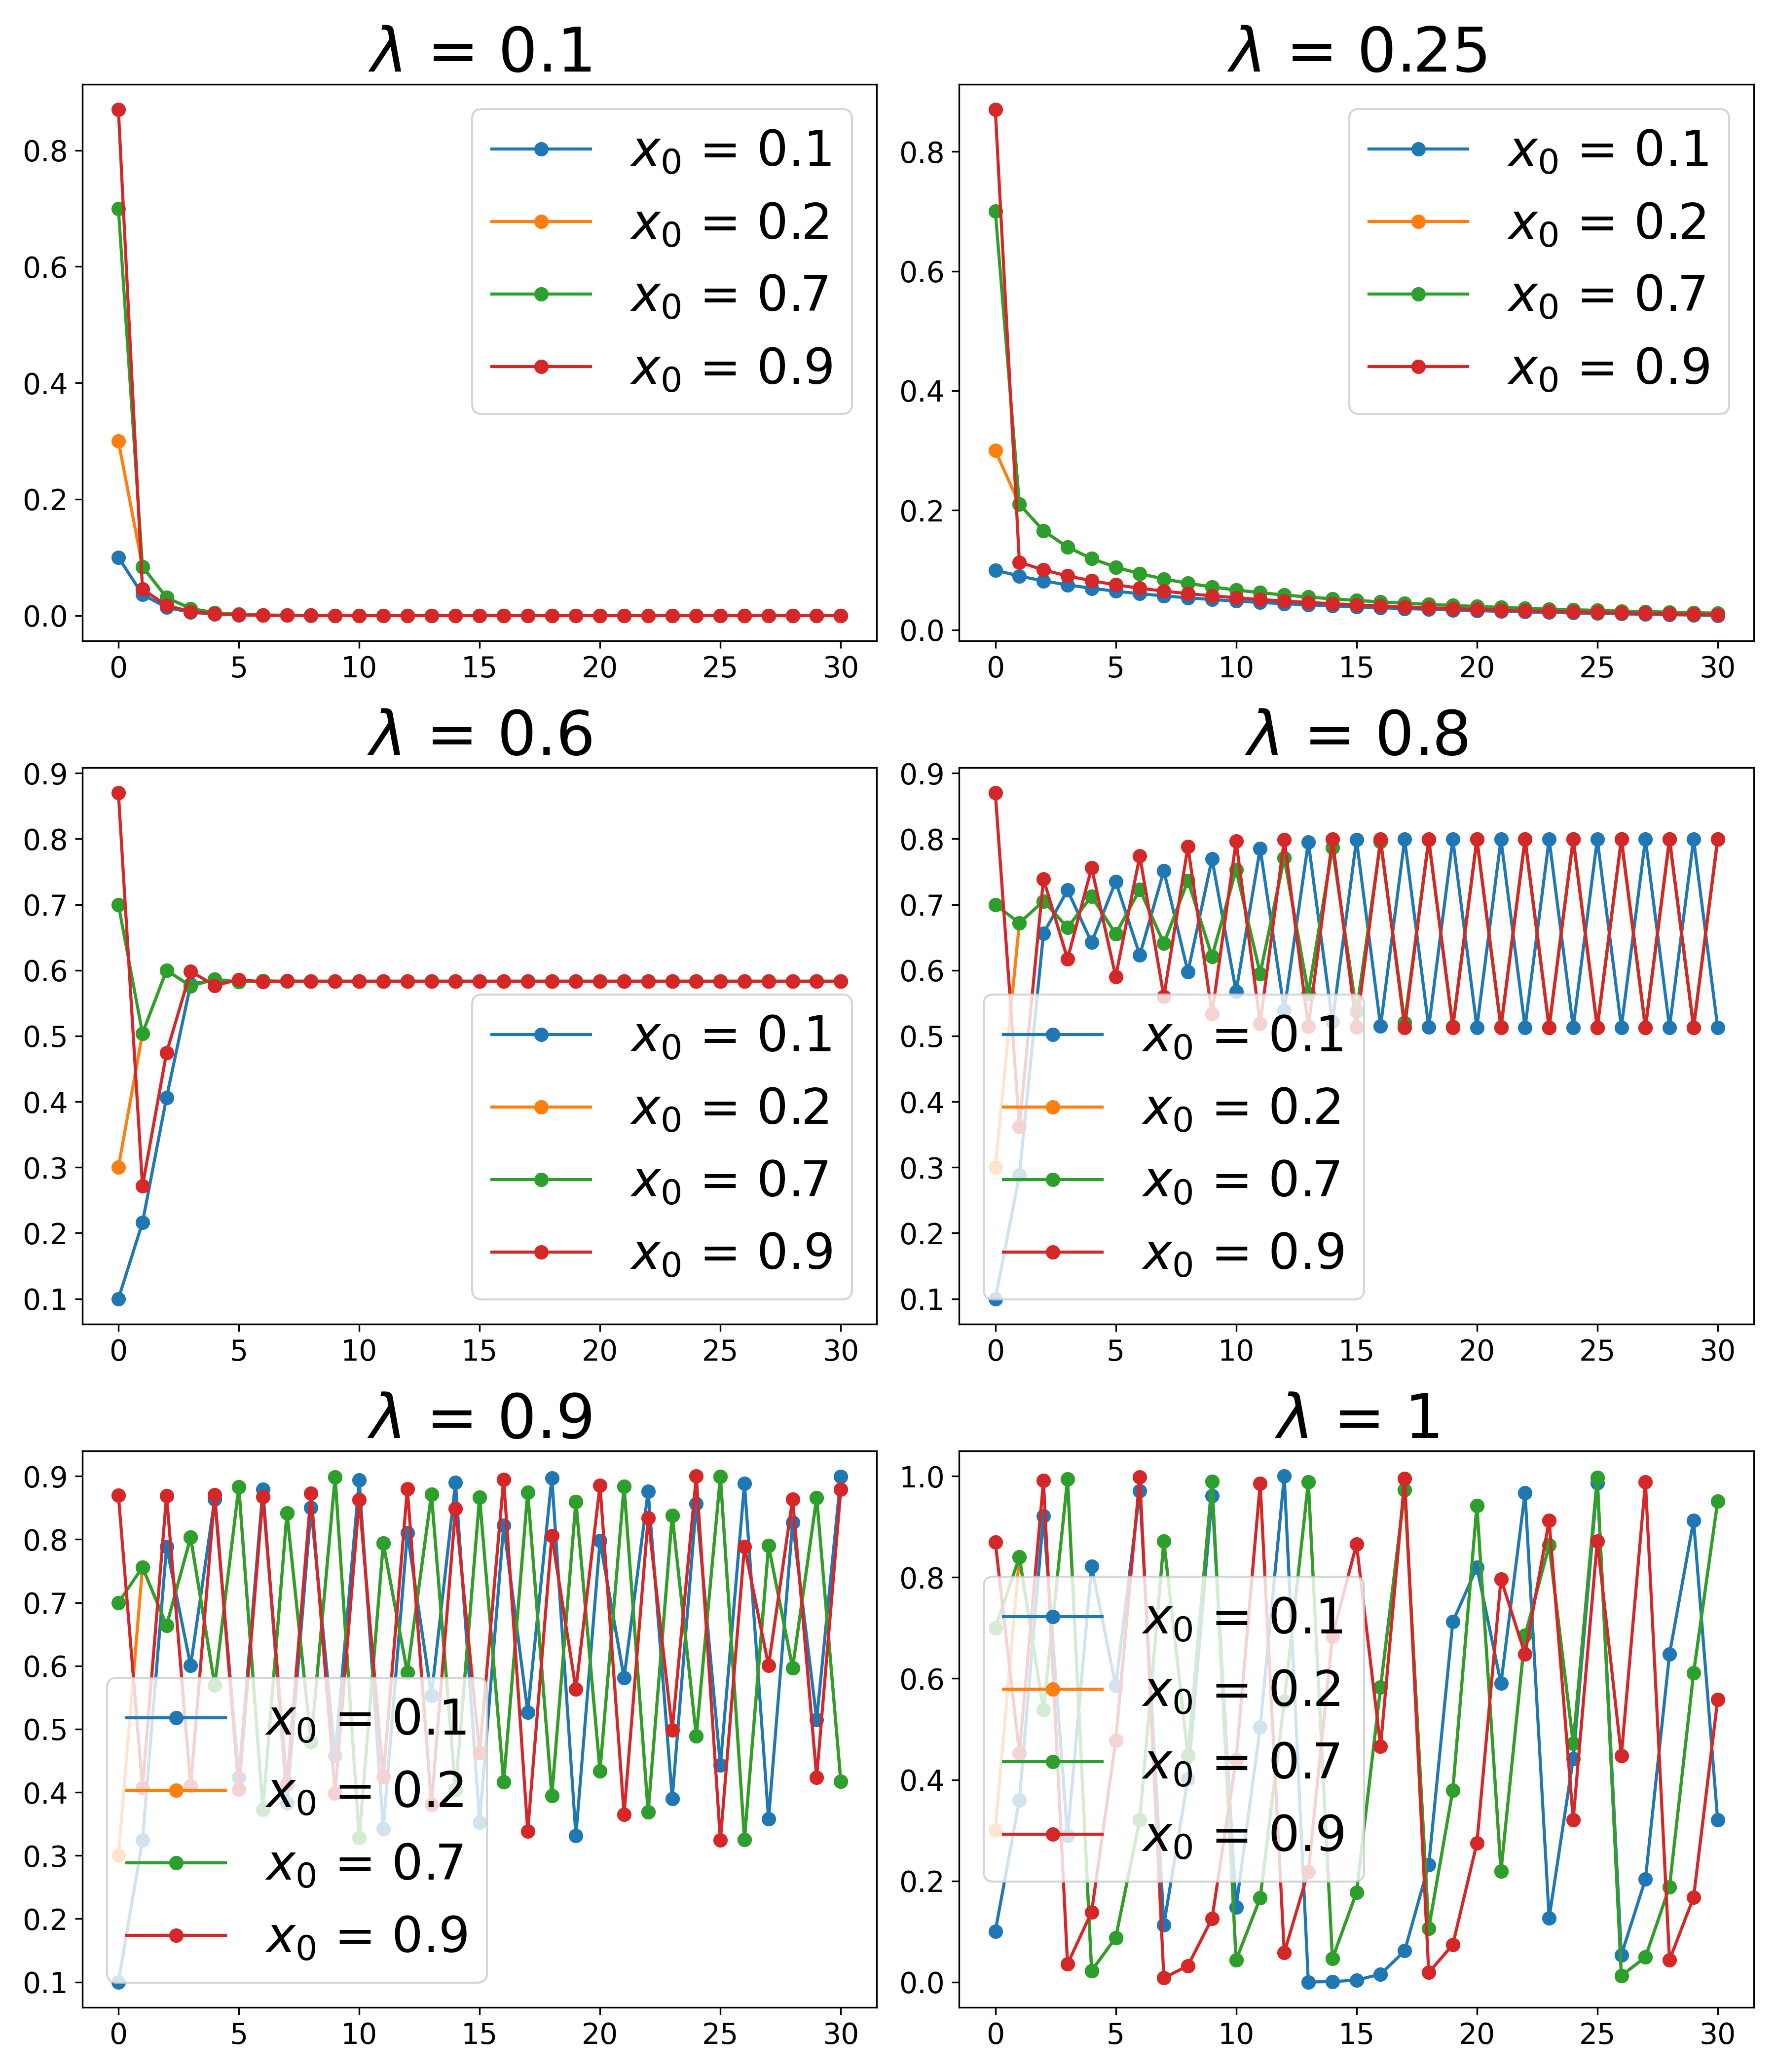
\includegraphics[width=\textwidth]{./figures/various_iterating_logistic_map.png}
	\caption{Iterating the logistic map with different initial values and $\lambda$. All graphs are produced by setting a $x_0$ and $\lambda$, and iterating $x_{n+1} = L_{\lambda}(x_n)$, and plotting all $x_n$ values respect to iteration number $n$.}
\end{figure}

There are several immediate observations upon looking at the figure \ref{fig:various_iter_logistic}.
When $\lambda = 0.1$ and $0.25$, it seems $\lim_{n \rightarrow \infty} x_n = 0$ regardless of the value of $x_0$.
For $\lambda = 0.6$, $\lim_{n \rightarrow \infty} x_n = l \neq 0$. 
(We can show that, after more tools are developped in the next sessions, $l = \frac{7}{12}$). 

When $\lambda = 0.8$, $x_n$ no longer converges but oscillates in a stable two orbit. 
For $\lambda = 0.9$ and $\lambda = 1$, it is not clear that if $x_n$ has any stable orbits or sensible patterns, and the best epithed for them would be `chaotic'.
A rigorous topological definition for chaos will be provided in the following session. 
% TODO: add which session

For all cases it seems like any initial condtion, $x_0$, upon iteration, will eventually tend to some common dynamical behavior depending only on $\lambda$.
The scatter plot, figure \ref{fig:logistic bifurcation overview}, is produced to capture the behavior of $x_n$ as $n \rightarrow \infty$ for $0 \leq \lambda \leq 1$. 
Two zoomed in figure around the area of interests are also produced in figure \ref{fig:logistic_bifurcation_zoom_1} and \ref{fig:logistic_bifurcation_zoom_2}.

These pictures are indeed spectacular. 
For $\lambda$ between $0$ and $a_0 = 0.25$, there is a stable fixed point $x = 0$.
When $\lambda$ increases and become greater than $a_1 = 0.75$, $0$ no longer the stable fixed point, but there is another unique stable fixed point elsewhere.
Precisely when this stable fix point becomes unstable around $\lambda = a_2 \approx 0.77$, a stable two cycles appears.
The stable two cycle, again, disappeared around $\lambda = a_3 \approx 0.86$, at which point a stable 4 cycles appears. 
This periodic doubling of orbits, which seems to continue indefinitely, is called bifurcation. 
Upon a closer inspections on figure \ref{fig:logistic_bifurcation_zoom_1} and figure \ref{fig:logistic_bifurcation_zoom_2}, each stable orbit seems to be self-similar, and all stable orbit cross the line $y = 0.5$ for some $\lambda$.

Bifurcation, however, does not exhaust the whole spectrum of $[0,1]$, and $a_{n}$ seems to converge to some limit as $n \rightarrow \infty$. 
Label this limit as $a_{\infty}$.
For $\lambda > a_{\infty}$, there are no longer any obvious pattern and the overall behavior is best described as chaotic. 
Nevertheless, in this chaotic region there are windows for stable orbits of odd periods which are not observed for $\lambda < a_{\infty}$. (The term window describing an interval of $\lambda$ for which stable orbit orbit exists is introduced by May \cite{May_Nature}.)
Examples are $\lambda \approx 0.957$ for a 3-cycle and $\lambda \approx 0.934$ for a 5-cycle in figure \ref{fig:logistic_bifurcation_zoom_3}.

The following paragraph listes some of our observations and the sketch their proofs.

\begin{figure}[htbp]
	\centering
	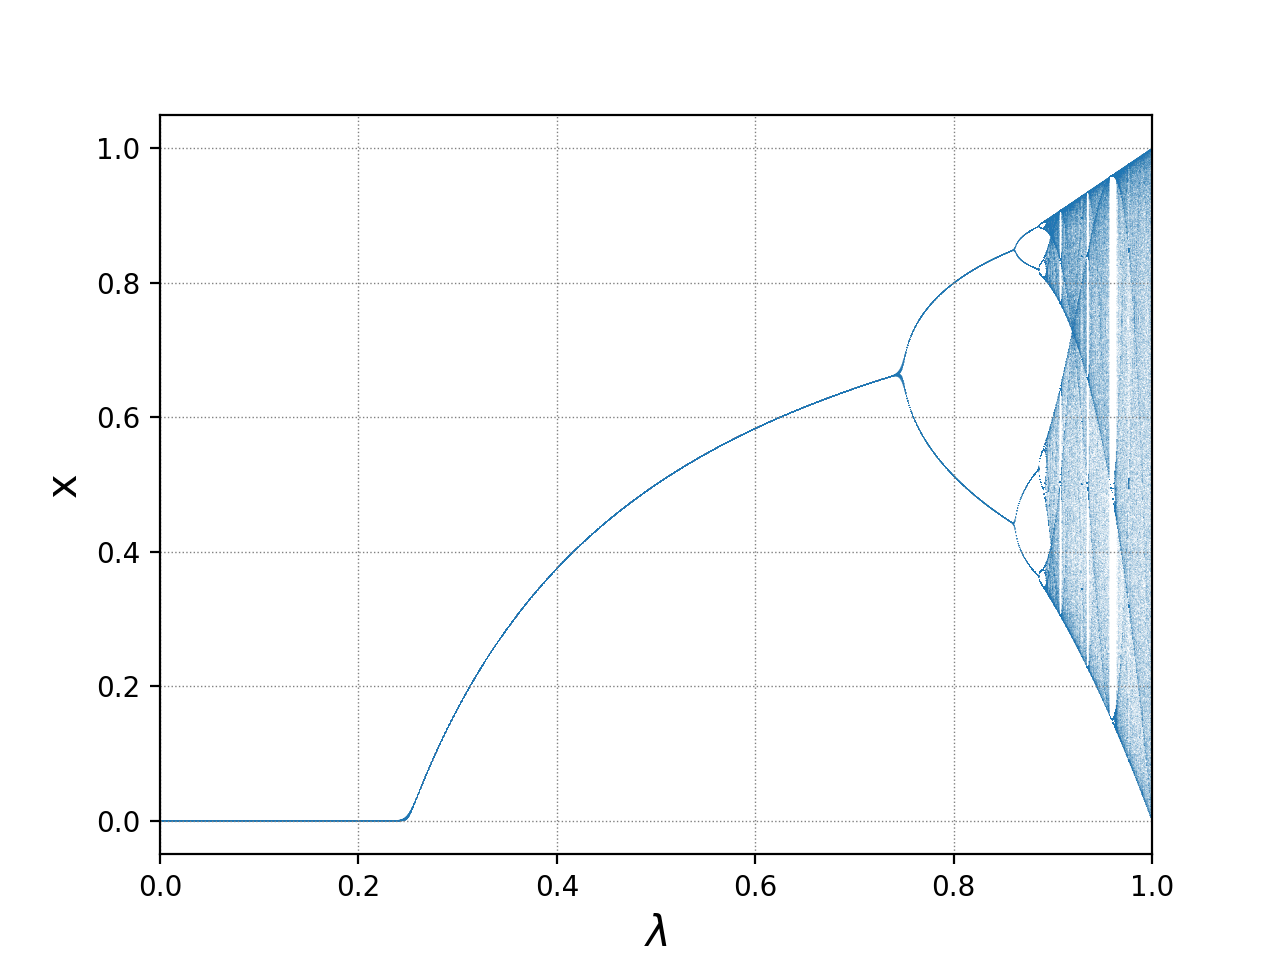
\includegraphics[width=\textwidth]{./figures/l_bifurcation_overview.png}
	\caption{For each $\lambda \in [0,1]$, $x_0$ is set to $0.5$, and the value of each iteration of $x_{n+1} = L_{\lambda}(x_n)$ was plotted at the coordinate $(\lambda, x_{n+1})$ as a faint blue dot. 
	The first 100 iteration was discarded, and 1500 iterations were plotted for each value of $\lambda$.}
	\label{fig:logistic bifurcation overview}
\end{figure}

\begin{figure}[htbp]
	\centering
	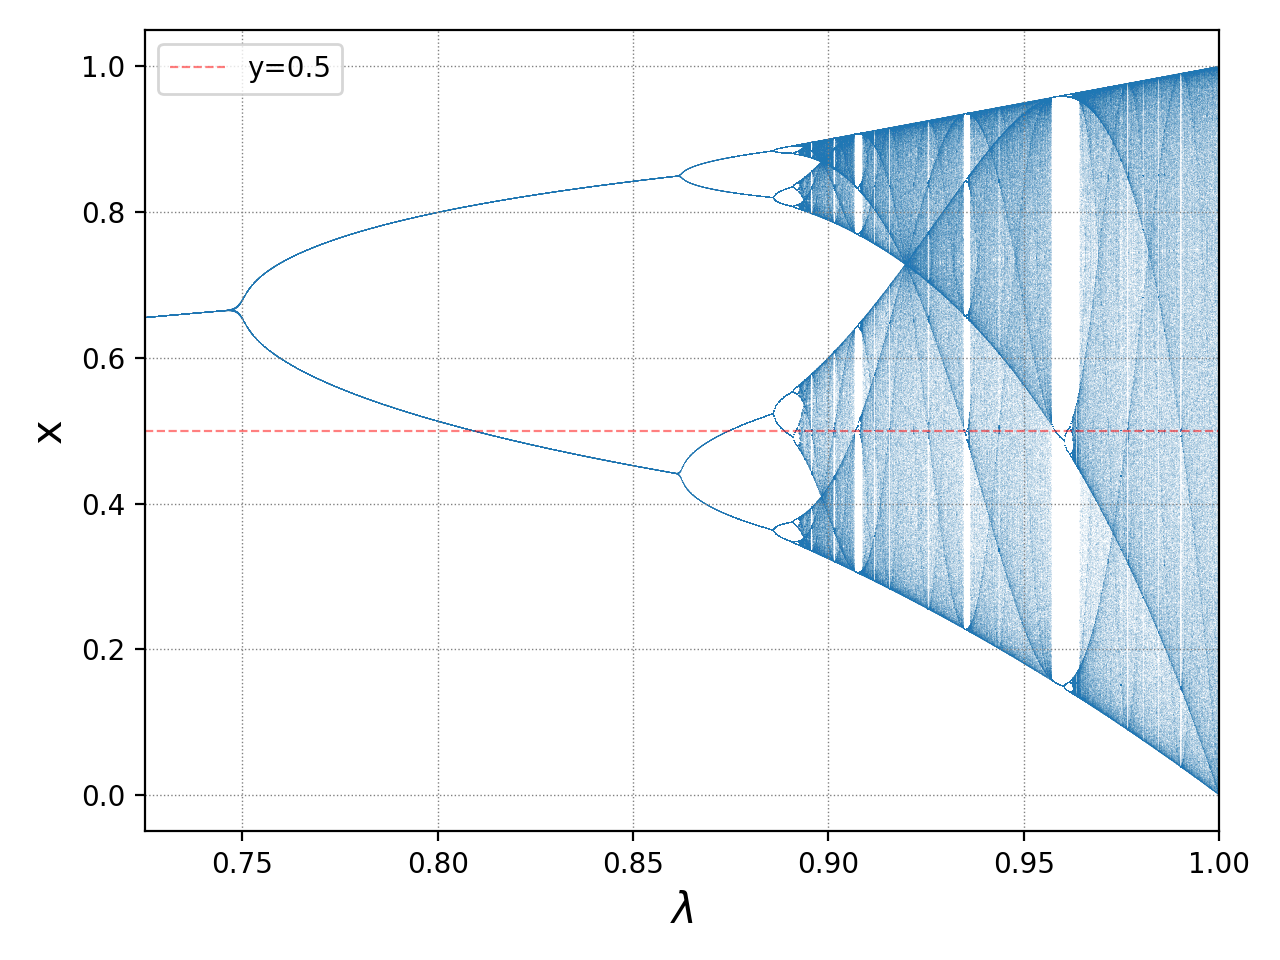
\includegraphics[width=\textwidth]{./figures/l_bifurcation_zoom_1.png}
	\caption{Zooming in the figure \ref{fig:logistic bifurcation overview} at the interval $0.5 \leq \lambda \leq 1$.}
	\label{fig:logistic_bifurcation_zoom_1}
\end{figure}

\begin{figure}[htbp]
	\centering
	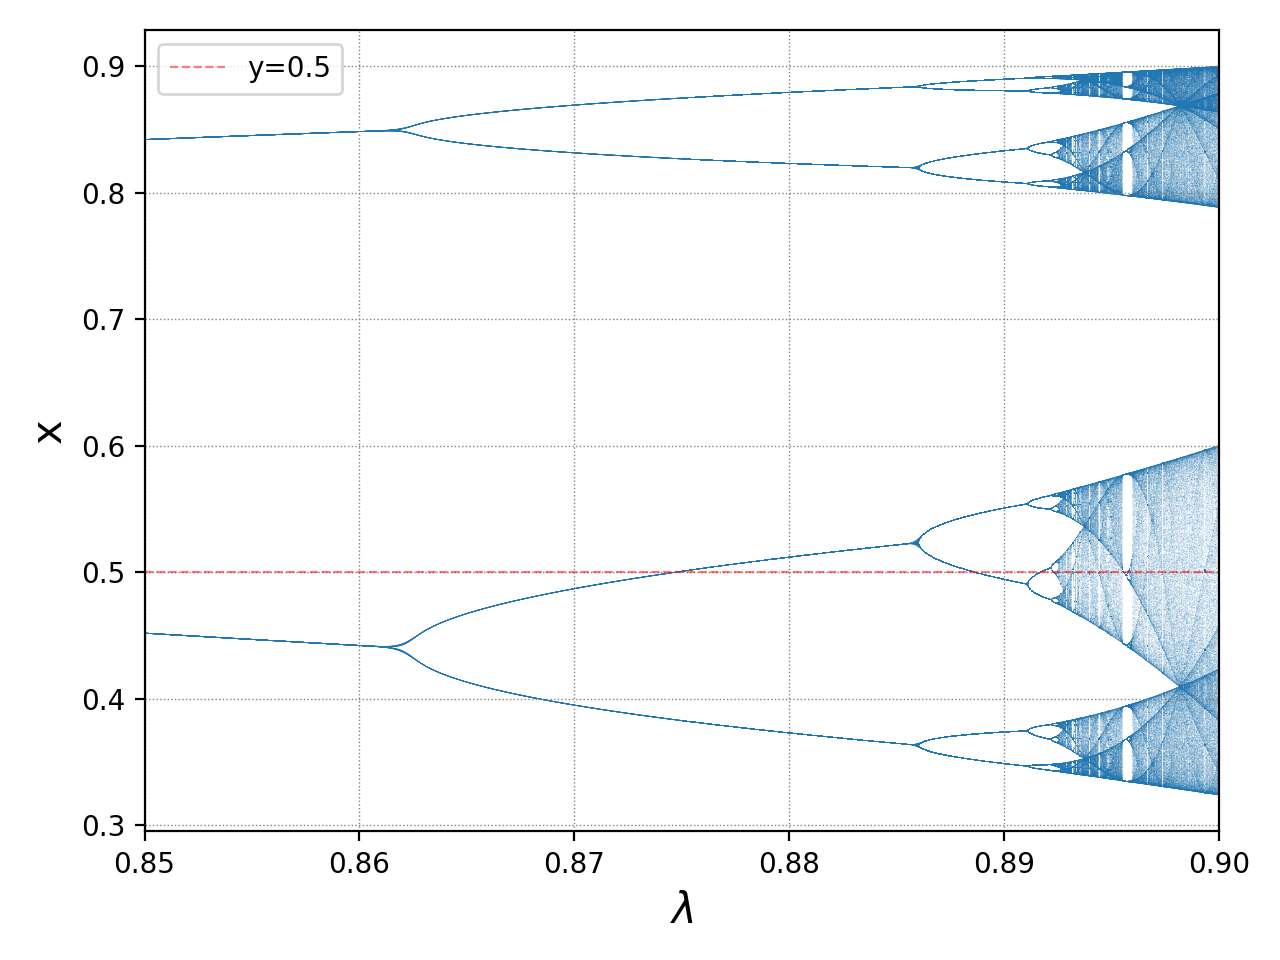
\includegraphics[width=\textwidth]{./figures/l_bifurcation_zoom_2.png}
	\caption{Zooming in the figure \ref{fig:logistic bifurcation overview} at the interval $0.85 \leq \lambda \leq 9$.}
	\label{fig:logistic_bifurcation_zoom_2}
\end{figure}

\begin{figure}[htbp]
	\centering
	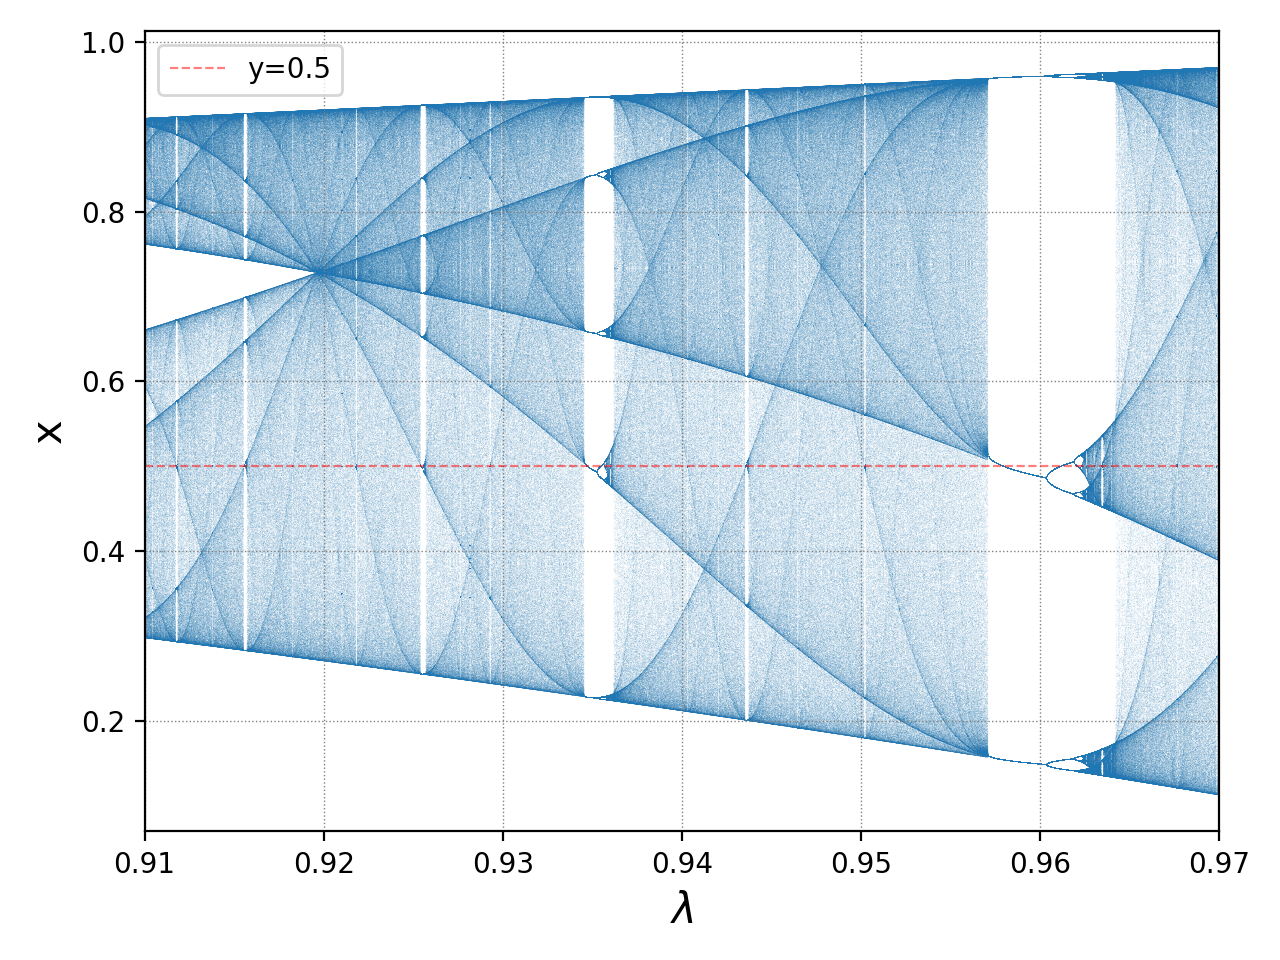
\includegraphics[width=\textwidth]{./figures/l_bifurcation_zoom_3.png}
	\caption{Zooming into figure \ref{fig:logistic bifurcation overview} in chaotic region}
	\label{fig:logistic_bifurcation_zoom_3}
\end{figure}

\begin{observation}[Logistic Bifurcation]\label{th:logistic_bifurcation}
	Let $L_{\lambda} = \lambda 4x(1-x) $ be the logistic function as defined in \ref{eq_logistic}.

	\begin{enumerate}
		\item For $0 < \lambda < a_0 = \frac{1}{4}$, the system has one unique fixed point at $x = 0$. \label{log_fix_0}

		\item For $a_0 <\lambda < a_1 = \frac{3}{4}$, the fixed at $x=0$ is no longer stable, but a new stable one-cycle were developped. \label{log_fix_1}

		\item When $\lambda$ becomes greater than some value $a_2$, the one cycle is no longer stable. 
		Precisely at the point when the one cycle fails to be stable, a stable two cycle appears. 
		Similarly, the 2 cycle will bifurcated into 4 cycles at $a_3$, $2^n$ cycle to $2^{n+1}$ cycle etc, until $\lambda > a_{\infty}$. 
		\label{log_periodic_doubling}
		\item Specifically, for any $\lambda$ there is at most one set of stable orbits. \label{log_at_most_one_stable_orbit}

		\item Let $[a, b]$ be a window of stable orbit of period $n$.
		There exists $\epsilon \in [a, b]$ such that $L_{\epsilon}^n(0.5) = 0.5$. 
		This is the intuitive observation that every orbit must cross the line $x = 0.5$, as shown in figure \ref{fig:logistic_bifurcation_zoom_1} and \ref{fig:logistic_bifurcation_zoom_2}. \label{log_cross_half}

	\item \label{log_simul_stable_or_unstable}
		Assume for certain $\lambda$ there is an $n$ cycle. That is, there exists distinct $x_1, \cdots, x_n$ such that $\L(x_1) = \L(x_2), \L(x_2) = \L(x_3) \cdots \L(x_n) = \L(x_1)$.
		Then necessarily $x_1, \cdots, x_n$ are $n$ fixed points of $\L^n$. 
		These $n$ distinct fixed point for $\L^n$ and $\lambda$ must be simultaneously attacting fixed points or repelling fixed points, possibly except for a set of measure zero.

		\item  \label{log_chaos_at_1}
			When $\lambda = 1$, the map exhibit chaotic behavior defined in \ref{def:Devaney_definition_for_chaos}. 
	\end{enumerate}
\end{observation}

\begin{figure}[htbp]
	\centering
	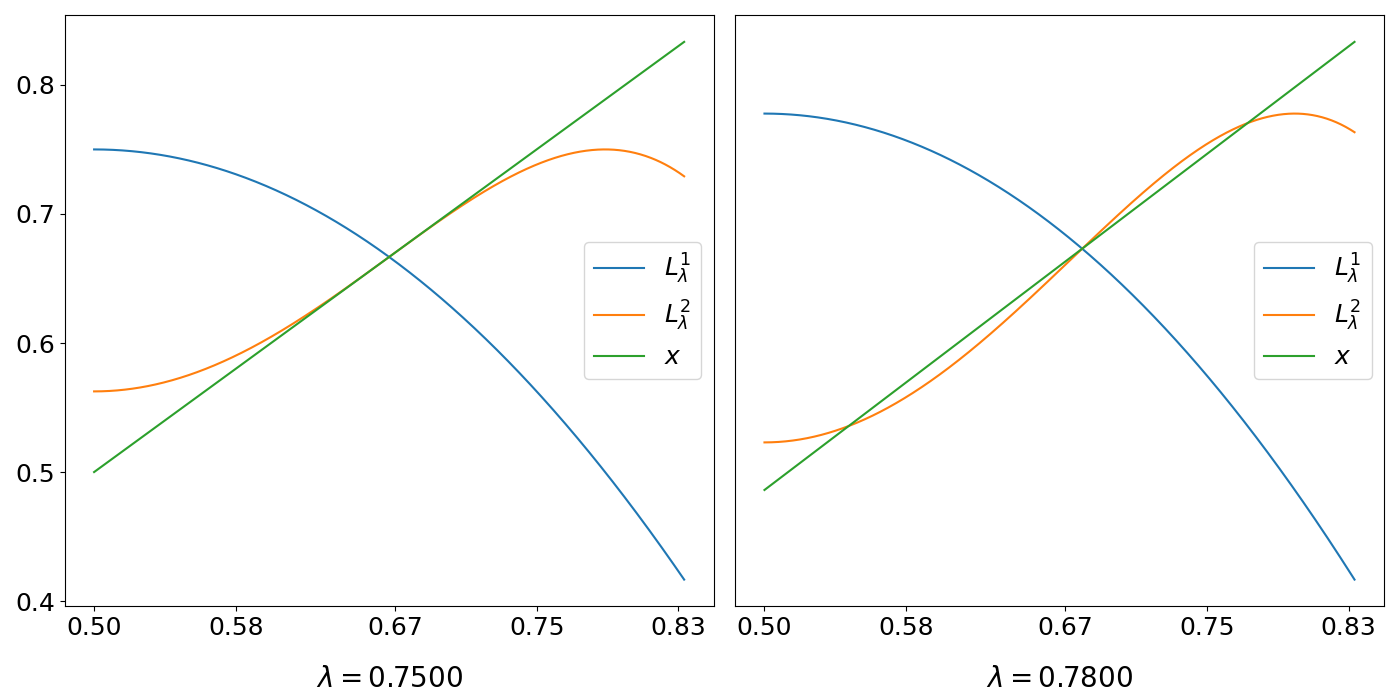
\includegraphics[width=0.8\textwidth]{./figures/logistic_map_around_bifurcation.png}
	\caption{
		$\L, \L^2$ and function $y=x$ are graphed and zoomed in around the fixed point for $\lambda = 0.75$ and $\lambda = 0.78$, where bifurcation takes place.
		For $\lambda < 0.75$, as can be seen from figure \ref{fig:logistic_bifurcation_zoom_1}, the system as a unique stable point,
		which loses its stability and a stable two orbit appears after $\lambda$ just increases above $0.75$.
		This is because, as shown on the right, precisely when the stable fixed point became unstable, the graph of $\L^2$ will have two more intersection with the line $y=x$, which becomes the stable two orbit.
	}
	\label{fig:point_of_bifurcation1}
\end{figure}

\begin{proof}[Proof of \ref{th:logistic_bifurcation}.\ref{log_fix_0} and \ref{th:logistic_bifurcation}.\ref{log_fix_1}]
	The fix point for $\L(x)$ is exactly the solution of the equation $\L(x) = x$, which are $x_0 = 0$ and $x_1 = 1 - \frac{1}{4\lambda}$. 
	$|L_{\lambda}(x_0) | = 4 \lambda < 1$ for $0 < \lambda < \frac{1}{4}$, so by theorem \ref{th:_stable_unstable_fixed_point} in these interval $x_0$ is a stable fixed point.
	Arguments for $x_1$ is similar.
\end{proof}


\begin{proof}[Demonstration of \ref{th:logistic_bifurcation}.\ref{log_periodic_doubling}]
	The proof of this phenomenon again exploits theorem \ref{th:_stable_unstable_fixed_point}.

	Let us concentration on $\lambda^*$ at which the fixed point $a$ becomes unstable, that is $L_{\lambda*}' a  = - 1$ and when for any $\lambda > \lambda^*$, the derivative at the fixed point being smaller than $-1$, thus $a$ becomes an unstable fixed point. (This observation is made obvious in figure \ref{fig:point_of_bifurcation1}.)
	Necessarily, $\frac{d}{dx}L_{\lambda^*}^2 a = L'_{\lambda^*}(a) \cdot L'_{\lambda^*}(a) = 1$,
	and for any $\lambda > \lambda^*$, $\frac{d}{dx}L_{\lambda}^2a'> 1$, where $a'$ is the new fixed point.

	Since $\frac{d}{dx}L_{\lambda}^2(a') > 1$ for some $\delta > 0$, $\L^2(a' - \delta) < a' - \delta$, and $\L^2(a' + \delta) > a' + \delta$. 
	Observe that $\L^2(1) = 0 < 1$, so by intermediate value theorem there must be some point $b > a' + \delta$ such that $\L^2(b) = b$. 
	Around $a'$ $L^2$ is concaving upwards, meaning its derivative is decreasing, this means that $\frac{d}{dx }L_{\lambda}^2(b) < 1$,
	and we can pick some $\lambda$  close to $\lambda ^*$ such that $-1<\frac{d}{dx }L_{\lambda}^2(b) < 1$, and at this point $b$ is a stable fixed point of $L_{\lambda}^2$.
	The argument for the other fixed point smaller than $a'$ is similar. 

	Although our arguments are qualitative, it can be made precise and rigourous by the use of Schwarzian derivative, as shown in chapter 12 of \cite{Devaney_green_book_chaos_definition}.
\end{proof}

\begin{proof}[Demonstration of \ref{th:logistic_bifurcation}.\ref{log_at_most_one_stable_orbit}]
	This follows from the previous point, but also stems from the fact that $\L^n$ is a function of negative Schwarzian derivative with bounded interval for stable points.
	The number of stable orbits of such maps must not exceed the number of critical points.

	This fact is proved in \cite{Pierre_Collet} and in chapter 11 of \cite{Devaney_green_book_chaos_definition}.
\end{proof}

\begin{proof}[Proof of \ref{th:logistic_bifurcation}.\ref{log_cross_half}]
	As shown in theorem \ref{th:_stable_unstable_fixed_point}, a fixed point $x$ of the iterated map $f$ will be stable if $|f'(x)| < 1$ and unstable if $|f'(x)| > 1$.
	By chain rule, 
	$\frac{d}{dx}\L^2 (x) = \L'(\L(x))\L'(x)$, and similarly
	$$
		\frac{d}{dx} L_{\lambda}(x)^n = \L'(x)\prod_{i=1}^{n-1} L_{\lambda}'(L_{\lambda}^i(x))
	$$

	Since $x_0 = 0.5$ is the local maximum of $\L(x)$, the above equation shows that at $x_0 = 0.5$ $\frac{d}{dx} \L^n(x) = 0$ for all $n$.
	This means if $x_0$ is a fixed point of $\L^n(x)$, it will necessarily be stable. 
	
	To show that for each $n$, there exist a $\lambda$ such that $\L^n(x_0) = x_0$ is straightforward. 
	Notice at $\lambda = 0, \L^n(0.5) = 0$, and at $\lambda = 1, \L^n(0.5) = 1$.
	$\L^n(x)$ is a continuous function when regarding as a function of $\lambda$, so by intermediate value theorem there must be some $\lambda$ such that $\L^n(0.5) = 0.5$.
\end{proof}

\begin{proof}[Proof of \ref{th:logistic_bifurcation}.\ref{log_simul_stable_or_unstable}]
		Assuming there exists distinct $x_1, \cdots, x_n$ such that $\L(x_1) = \L(x_2), \L(x_2) = \L(x_3), \cdots $, and $\L(x_n) = \L(x_1)$.

		Differentiate $\L^n$ and evalute at $x_1$ 
		$$
		\frac{d}{dx} \L^n(x_1) = \prod_{i=1}^n \L'(x_i)
		$$

		Indeed evaluting at any other $x_i$ gives the same value. 
		So except for a set of $\lambda$ such that $\frac{d}{dx} \L^n(x_1) = \pm 1$, these $n$ points regarding as fixed points of $\L^n$ must be simultaneously attracting or repelling fixed points by theorem \ref{th:_stable_unstable_fixed_point}.
\end{proof}

\begin{proof}[Proof of \ref{th:logistic_bifurcation}.\ref{log_chaos_at_1}]
	The doubling map \eqref{eq:doubling_map} is topologically conjugate to $L_{1}$, so $L_1$ is chaotic.
	This is proved in example \ref{ex_logistic_and_doubling}.
\end{proof}

\section{Feiganbaum's Constant}


\section{Single Nodal Functions Give Rise to Bifurcations}

\begin{defn}
	A function $f: [0,1] \rightarrow [0,1]$ is single nodal if 
	\begin{enumerate}
		\item $f$ is piecewise $C^2$, that is, doubly differentiable with continuous second derivative
		\item $f$ has a unique and differentiable maximum attained at $f(\mx) = 1$ and $f'$ is continuous at $\mx$.
% TODO: Do we need the condition that f has no other local maximum?
		\item $f(x) > 0$ and $f(1) = f(0) =0$
		\item $f(x)$ concave downwards, that is $f'' < 0$.
	\end{enumerate}

	This definition is modified from appendix A of Feigenbuam's paper \cite{F1}.
\end{defn}
